\section{Results}

Data from the US senate government \cite{voting} has been analyzed in order to find dependencies among politician during voting processes. The dataset consists on all the 2017 senate voting records which has 191 samples of 100 politicians stored in a vector $X \in \mathbb{R}^{100}$, where the first 46 entries are democrat members, the 2 following are independent senators and the rest 52 are republicans.

The computational covariance matrix has been fed to the ADMM algorithm for different regularization problems. In the figure \ref{fig:sparse} is represented the sparse pattern found for different values of $\lambda$, where white space means a zero entry. In one extreme, for $\lambda=0.3$ we see a diagonal matrix, where each politician vote completely independently. In the other extreme for $\lambda=0.001$ we see a dense inverse covariance matrix, where everyone depends on everyone else. However, for $\lambda=0.05$ and $0.01$ density is only present in first and fourth quadrant. This results suggest, as expected, that each politician vote depends on what their party fellows are voting. 

\begin{figure}[h]
	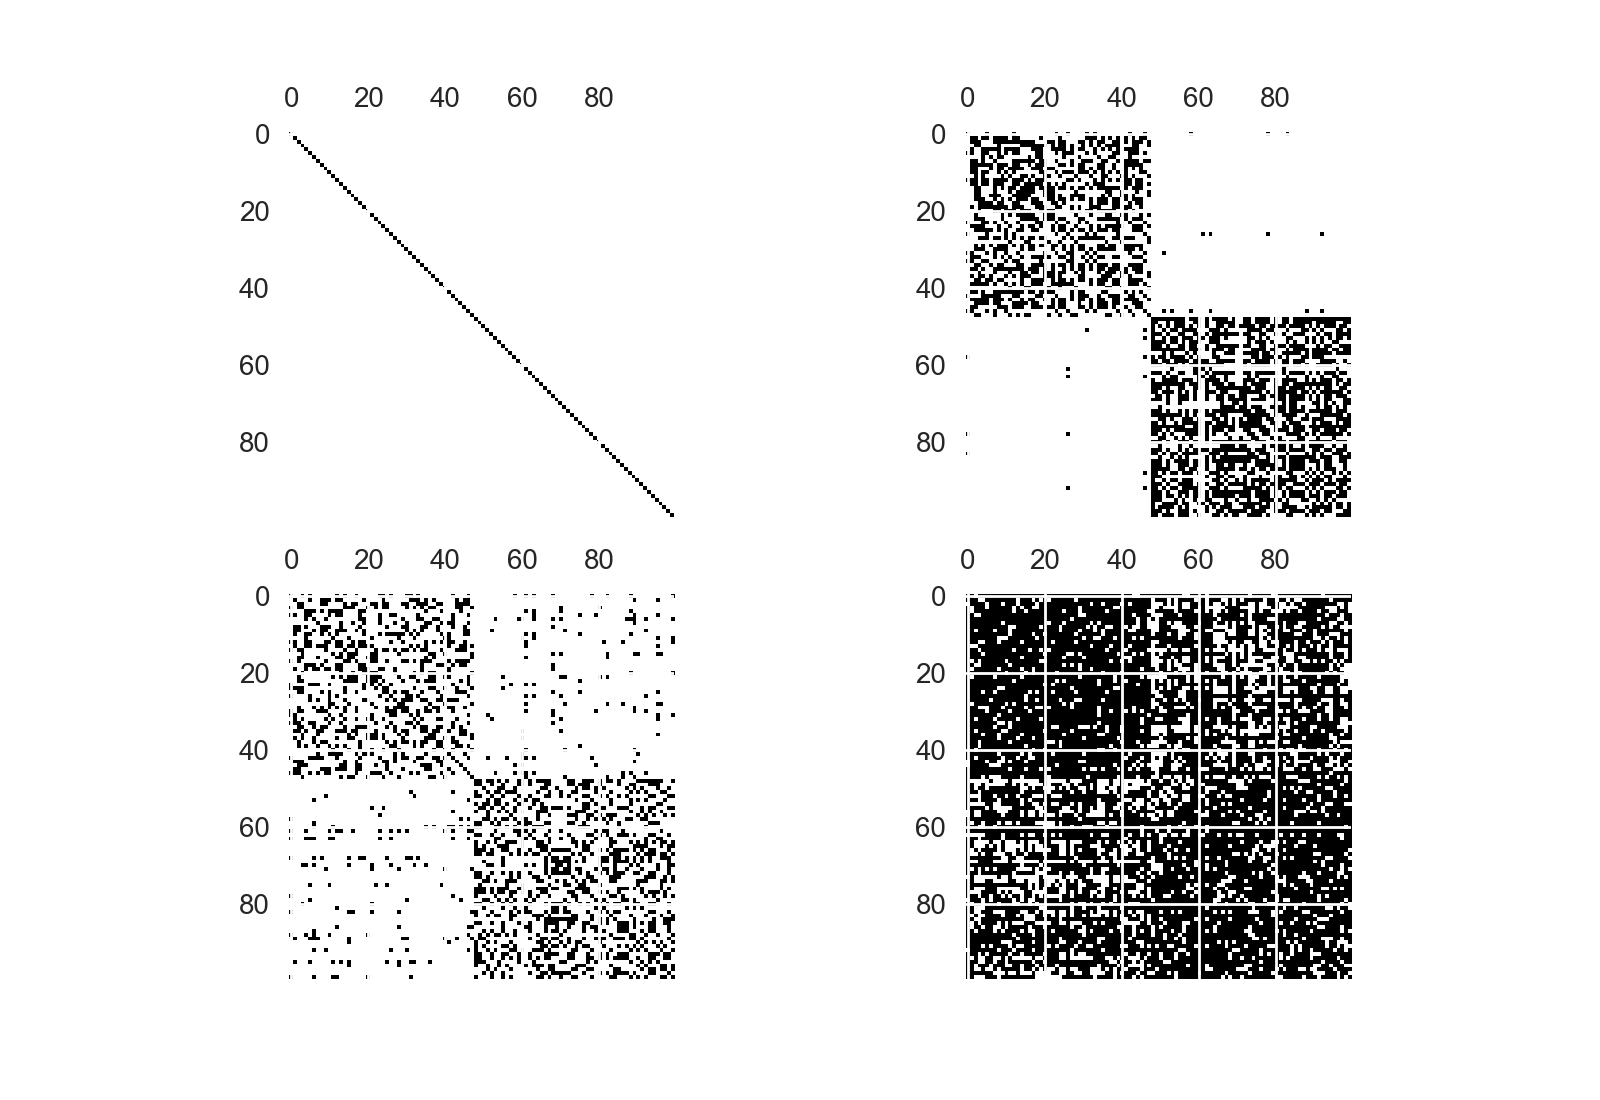
\includegraphics[width=1.1\textwidth]{figures/sparse_pattern.png}
	\caption{By order, sparse patterns for $\lambda$=0.3, 0.05, 0.01 and 0.001}
	\label{fig:sparse}
\end{figure}

The absolute and relative tolerance in (\ref{eq:ep_primal}) and (\ref{eq:ep_dual}) for all the experiments have been set to $10^{-3}$. The figure \ref{fig:convlambda} shows convergence of primal and dual residuals for different regularization values and fixed $\rho$. For $\lambda = 0.3$ it takes more time, since the relative tolerance is smaller, while for $\lambda = 0.001$ it takes longer since the residuals decrease slower.  
\begin{table}[h]
	\centering
	\begin{tabular}{l*{5}{c}r}
		Regularization($\lambda$)& 0.3 & 0.1 & 0.05 & 0.01 & 0.001 \\
		\hline
		Iterations & 224 & 47 & 40 & 96 & 152   \\
	\end{tabular}
	\label{tab:iterlambda}
	\caption{Number of iterations depending on $\lambda$}
\end{table}

\begin{figure}[H]
	\centering
	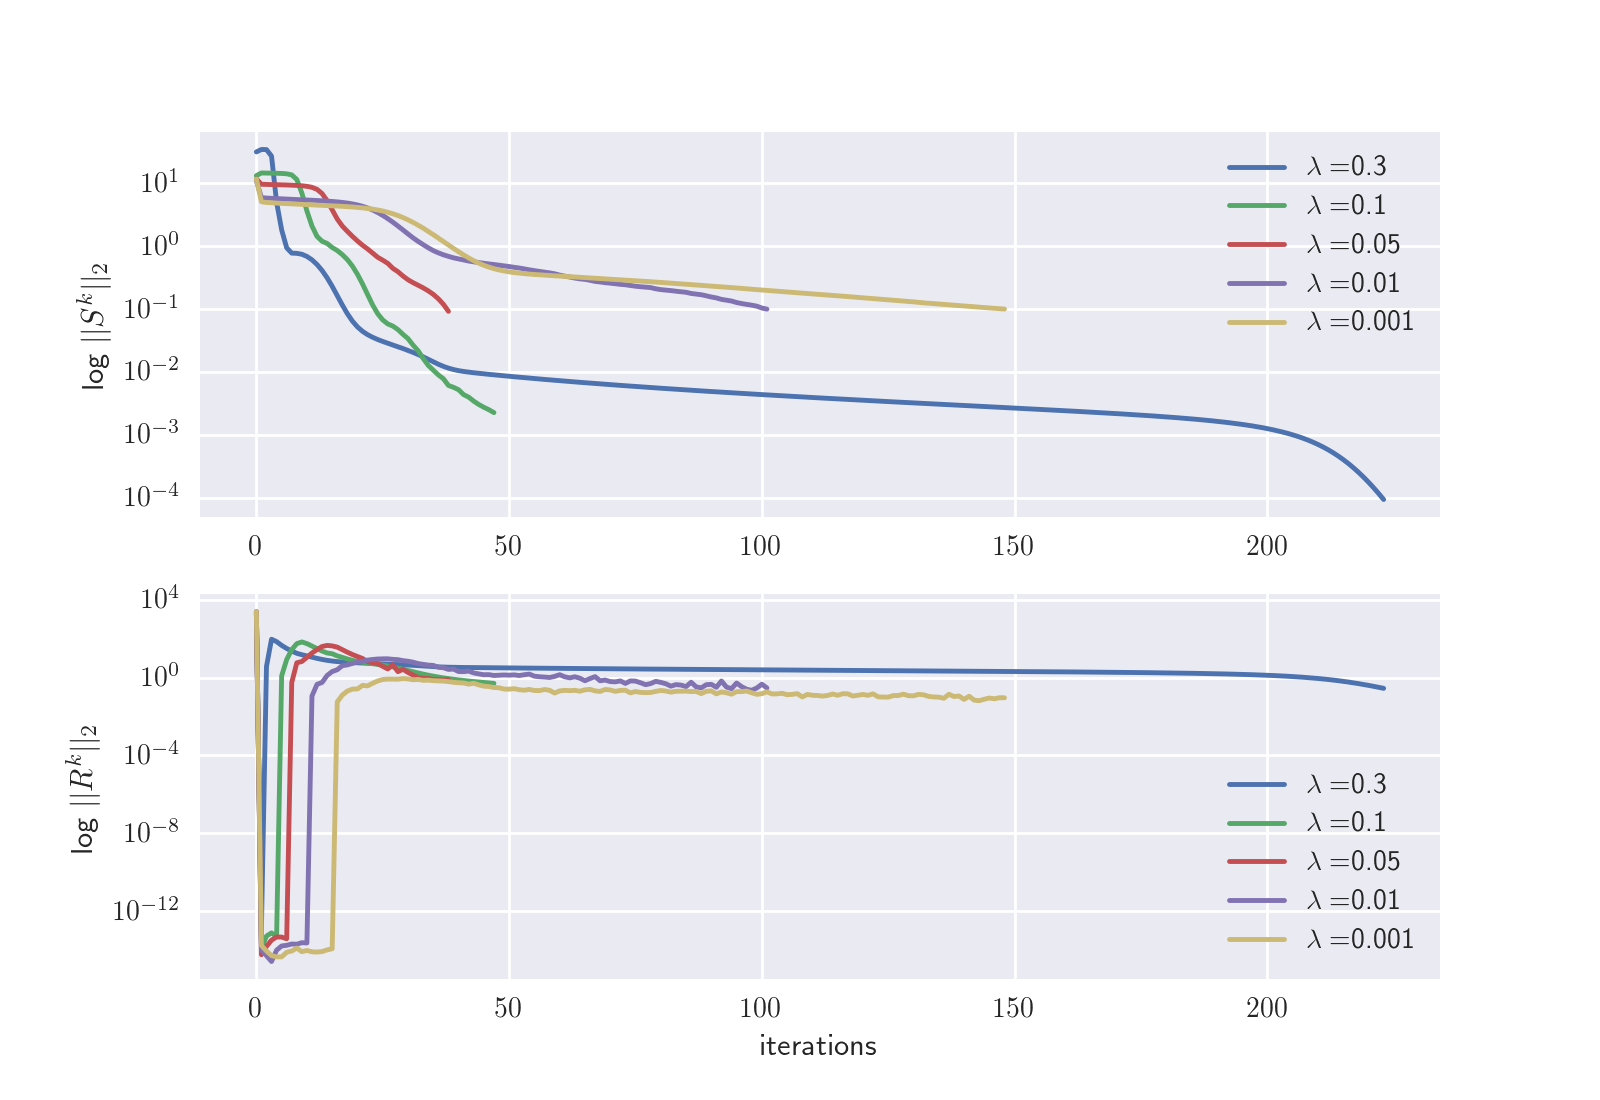
\includegraphics[width=\textwidth]{figures/convergence_lambda.png}
	\caption{Primal and Dual residuals convergence against $\lambda$ for fixed $\rho$}
	\label{fig:convlambda}
\end{figure}

The learning parameter, $\rho$, does not have impact on the accuracy of the solution but on the convergence speed. High values will decrease the dual function faster but the penalty for breaking primal feasibility will be high. In the figure \ref{fig:rhoiter}  we can see that the optimal point for $\lambda = 0.02$ is around 0.012.

\begin{figure}[H]
	\centering
	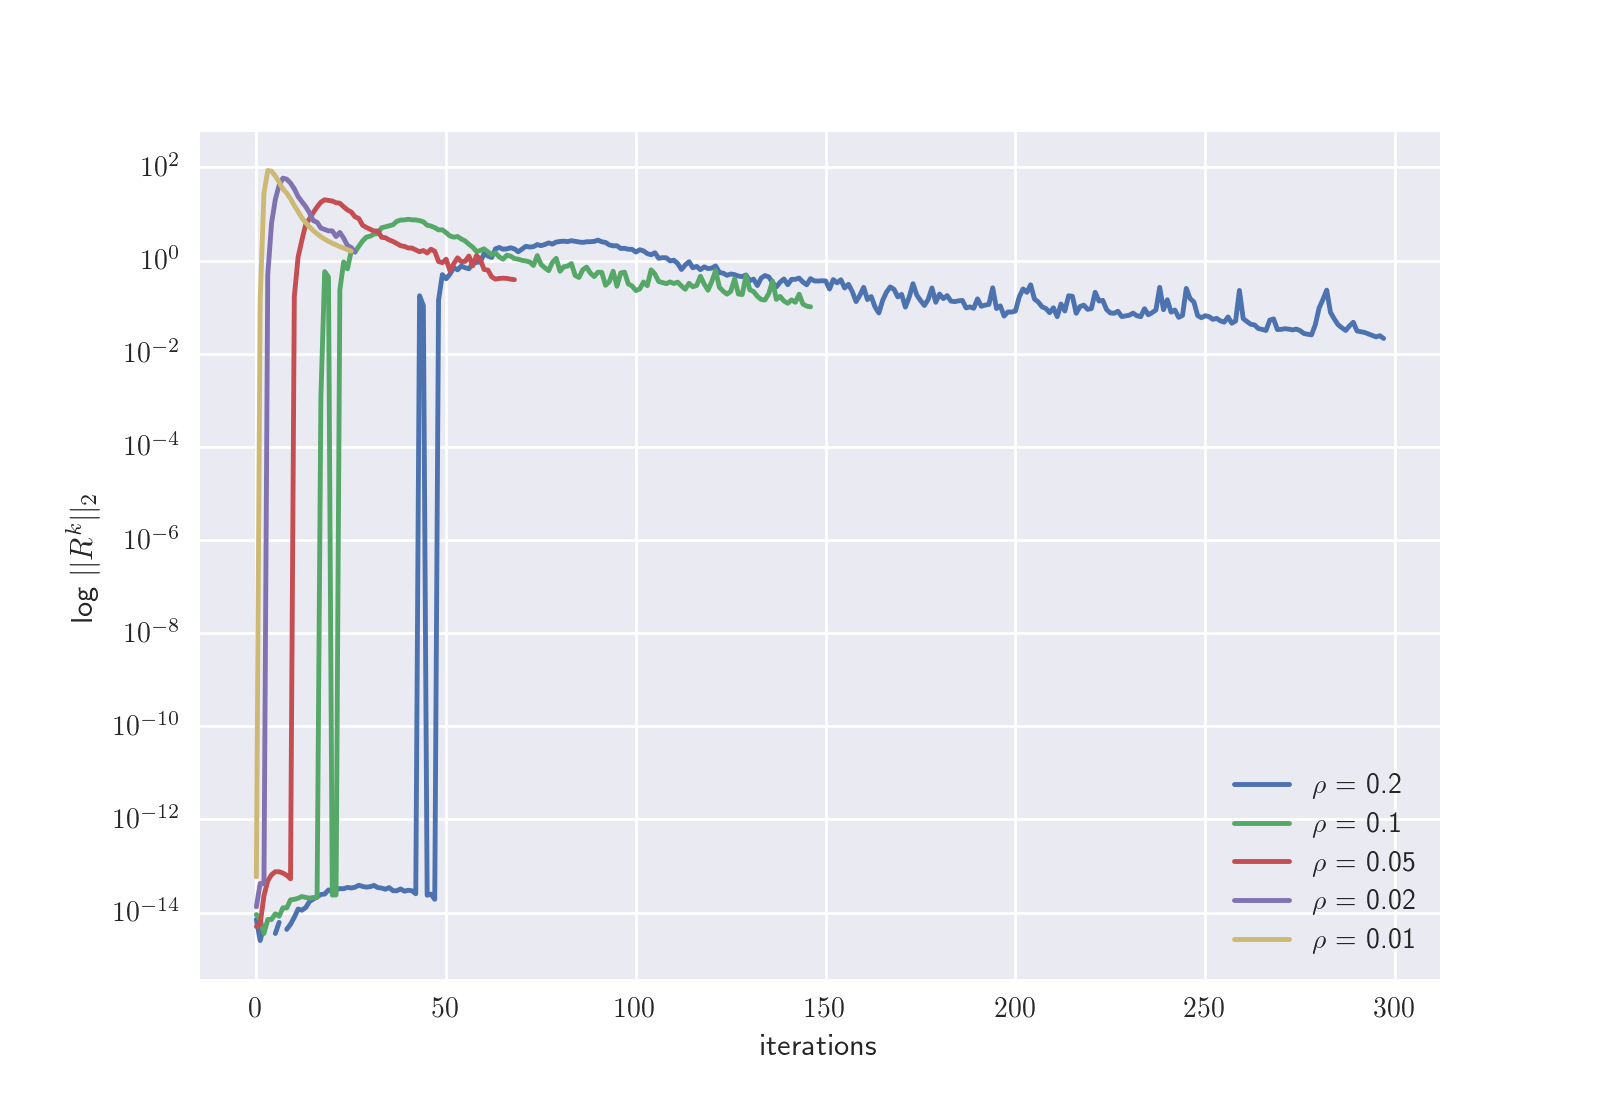
\includegraphics[width=\textwidth]{figures/convergence_rho.png}
	\caption{Primal residuals convergence against $\rho$ for $\lambda = 0.02$}
	\label{fig:convrho}
\end{figure}


\begin{figure}[H]
	\centering
	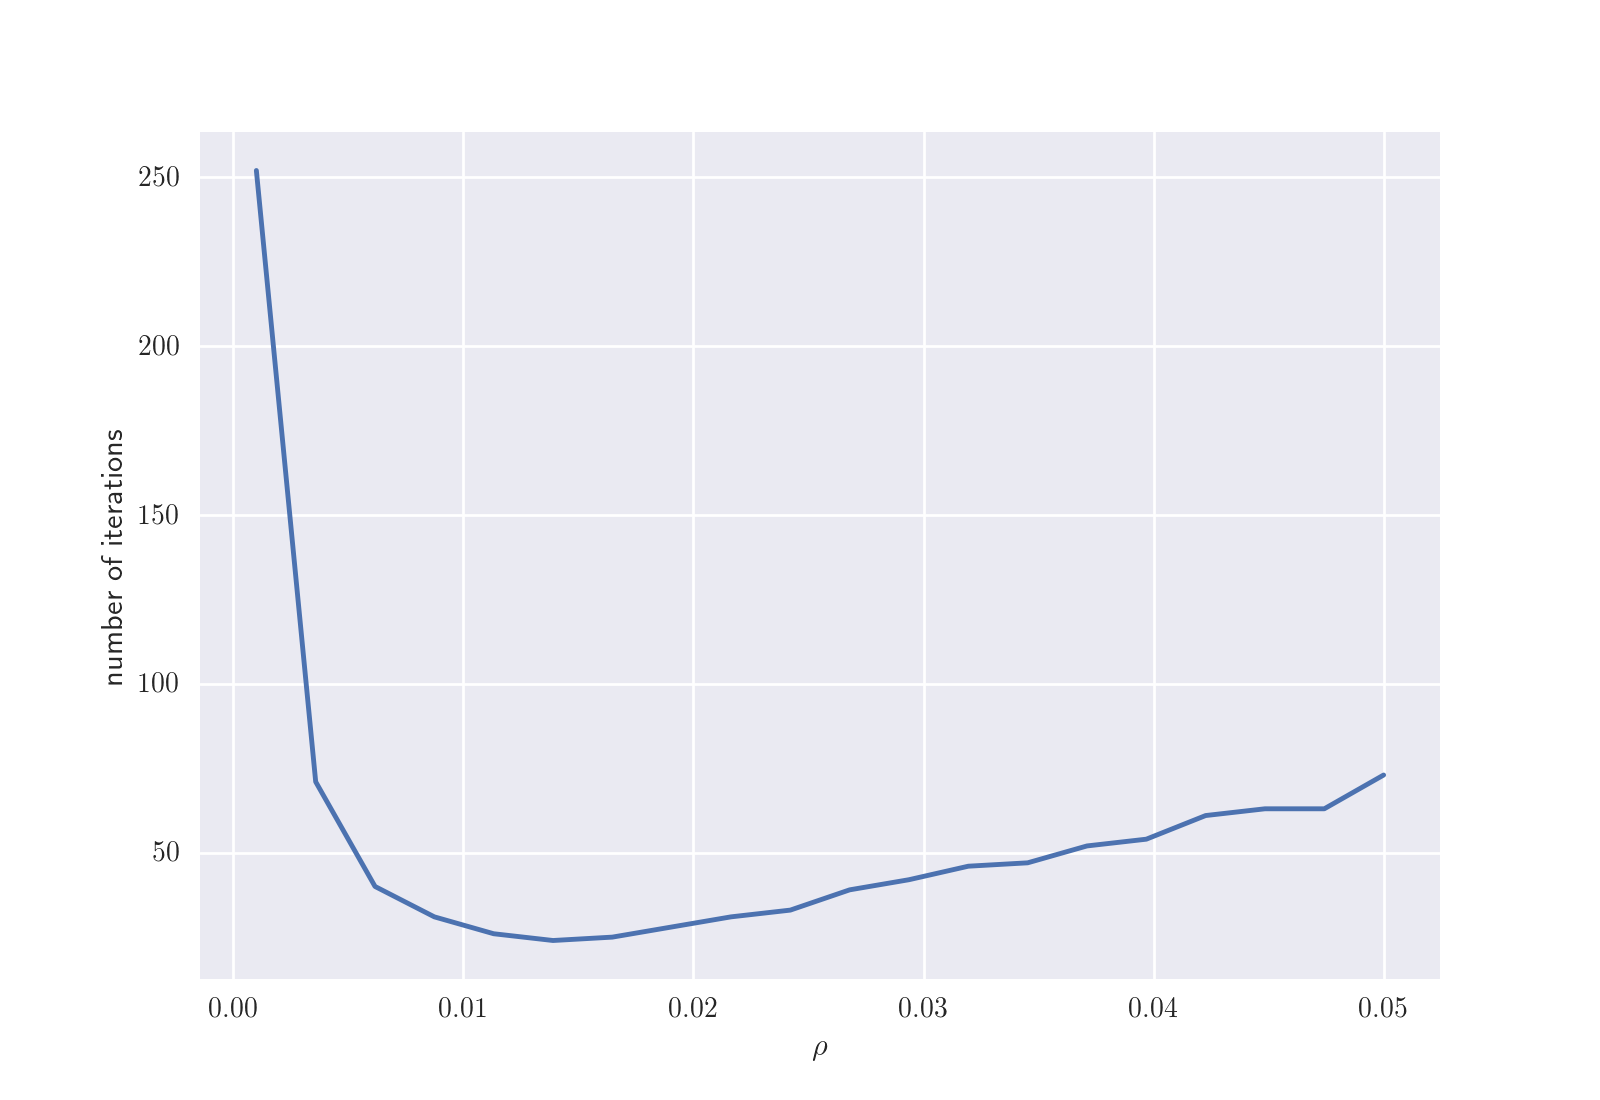
\includegraphics[width=\textwidth]{figures/rho_iter.png}
	\caption{Number of iterations against  $\rho$ for $\lambda = 0.02$}
	\label{fig:rhoiters}
\end{figure}
